\documentclass{article}

\usepackage{amsmath}
\usepackage{amssymb}
\usepackage{amsfonts}
\usepackage{mathtools}

\usepackage[thmmarks, amsmath]{ntheorem}

\usepackage{graphicx}
\usepackage{float}
\usepackage{tikz-cd}

\usepackage{diffcoeff}
\diffdef{}{op-symbol=\mathrm{d},op-order-sep=0mu}

\usepackage{cancel}
\usepackage{interval}

\usepackage{array}

\usepackage{enumitem}

\setlist[enumerate,1]{label=(\alph*)}

\title{Algebraic Topology Midterm}
\author{Duarte Maia}
%\date{}

\theoremstyle{plain}
\theorembodyfont{\upshape}
\theoremseparator{.}
\newtheorem{theorem}{Theorem}
\newtheorem{prop}{Prop}
\renewtheorem*{prop*}{Prop}
\newtheorem{lemma}{Lemma}
\newtheorem*{ex}{Exercise}

\theoremstyle{nonumberplain}
\theoremheaderfont{\itshape}
\theorembodyfont{\upshape}
\theoremseparator{:}
\theoremsymbol{\ensuremath{\blacksquare}}
\newtheorem{proof}{Proof}
\newtheorem{sol}{Solution}

\theoremsymbol{\text{\textit{(End proof of lemma)}}}
\newtheorem{lemmaproof}{Proof of lemma}

\newcommand{\R}{\mathbb{R}}
\newcommand{\C}{\mathbb{C}}
\newcommand{\Z}{\mathbb{Z}}
\newcommand{\Q}{\mathbb{Q}}

\newcommand{\RP}{\mathbb{RP}}

\newcommand{\kk}{\Bbbk}

\newcommand{\PP}{\mathbb{P}}
\newcommand{\FF}{\mathcal{F}}

\newcommand{\I}{\mathrm{i}}
\newcommand{\e}{\mathrm{e}}

\newcommand{\id}{\mathrm{id}}

\newcommand{\conj}[1]{\overline{#1}}
\newcommand{\close}[1]{\overline{#1}}

\DeclareMathOperator{\inte}{int}
\DeclareMathOperator{\codim}{codim}
\newcommand{\grad}{\nabla}


\DeclareMathOperator{\spec}{spec}

\DeclarePairedDelimiter{\abs}{\lvert}{\rvert}
\DeclarePairedDelimiter{\norm}{\lvert}{\rvert}
\DeclarePairedDelimiter{\Norm}{\lVert}{\rVert}
\DeclarePairedDelimiter{\braket}{\langle}{\rangle}


\begin{document}
\maketitle

\begin{ex}[1.2:16]
Show that the fundamental group of the surface of infinite genus is free on infinitely many generators.
\end{ex}

\begin{sol}
We endow this surface with the CW structure suggested by the following image.
\begin{figure}[H]
\centering
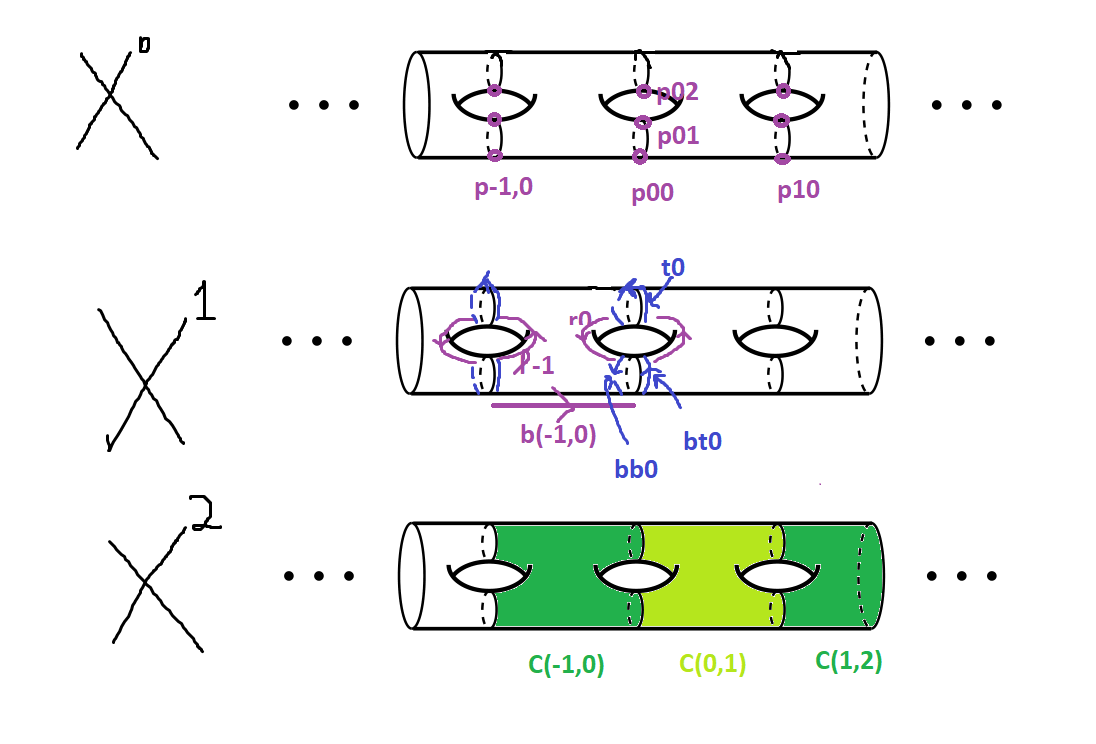
\includegraphics[width=\linewidth]{mt1}
\end{figure}

Now, we apply the recipe to compute the fundamental group of this image.

The first thing we need to do is fix a spanning tree of the graph $X^1$. Once we do, the generators of the fundamental group are (in one-to-one correspondence with) the edges of the graph which are not in this spanning tree. We choose the spanning tree given by all edges of the forms: $b_{i(i+1)}$, $bb_i$, and $r_i$. Therefore, the generators of the fundamental group are $t_{i(i+1)}$, $bt_i$, $\ell_i$, and $t_i$.

Now, the relations of the fundamental group are given by the two-cells. In this case, each cell $C(i,i+1)$ will furnish a relation between the generators $bt_i$, $bt_{i+1}$, $\ell_i$, $t_i$, and $t_{i+1}$. In order to understand what these relations are, we will now draw a cell $C(i,i+1)$ with its attaching map.
\begin{figure}[H]
\centering
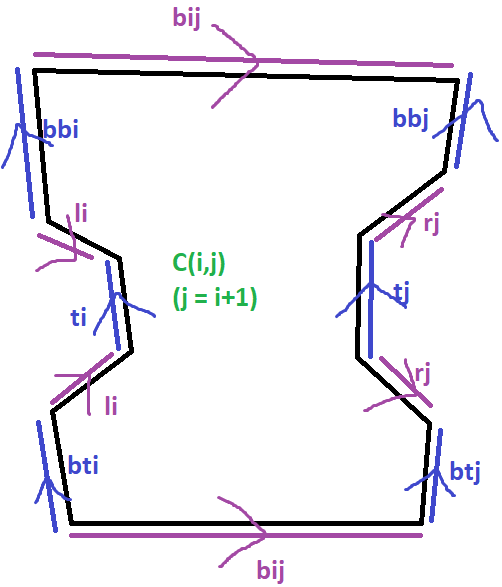
\includegraphics[width=5cm]{mt2}
\end{figure}

Now, each relation consists of going `around the attaching map' once, and identifying the resulting path with zero. We do this with this cell. Each edge in the spanning tree is ignored. The other edges correspond to their namesake generator. We obtain the relation: (with $j = i+1$)
\begin{equation} \label{eq:rels}
bt_j \, t_j \, \ell_i \, t_i^{-1} \, \ell_i^{-1} \, bt_i^{-1} = e.
\end{equation}

Now, this relation lets us write $bt_{i+1}$ in terms of the $t_j$, $\ell_j$, and in terms of $bt_i$, and the reverse could be done. Therefore, \emph{we may write all $bt_i$ in terms of the $t_j$, $\ell_j$, and $bt_0$}.\footnote{I could write the explicit expression, but I don't think it's necessary. To convince the reader that I know what I'm doing, however, I will sketch the expression for $bt_n$ with $n \geq 0$: $bt_n = bt_0 \ell_0 t_0 \ell_0^{-1} t_1 \dots \ell_{n-1} t_{n-1} \ell_{n-1}^{-1} t_n$.} This suggests that we consider instead these generators.

So, we consider the obvious map
\begin{equation}\label{eq:iso}
\braket{bt_0, t_i, \ell_i} \to \braket{bt_i, t_i, \ell_i \mid \eqref{eq:rels}}.
\end{equation}

We claim that this map is an isomorphism, because the inverse is well-defined. Indeed, to define the inverse, we need only take each $t_i$ and $\ell_i$ to itself, and each $bt_i$ to the expression that writes it in terms of the other generators. All that we need to show is that this correspondence respects the relations \eqref{eq:rels}; once we do we will have an inverse.

Showing that this correspondence respects \eqref{eq:rels} is trivially done by induction on $i$ (twice; once for positive $i$ and once for negative), and boils down to the fact that the expression we are sending each $bt_i$ to is precisely what makes \eqref{eq:rels} hold.

Since the map \eqref{eq:iso} is an isomorphism between a free group on countably many generators and a group which is isomorphic to the free group of the space under consideration, the exercise is solved.

\smallskip

Another way to see this solution: inductively we rewrite the equations \eqref{eq:rels} to all be of the form $bt_n = (\cdots)$, where the expression on the right-hand side depends only on the generators we've been discussing, and then we may simply remove all the generators $bt_n$, $n \neq 0$, together with the relations that tell us how to write them in terms of the others; this preserves the group up to isomorphism because adding generators and relations telling us how to write these generators in terms of the previous ones does not add any elements to the group.
\end{sol}

\begin{ex}[1.3:9]
Show that if a path-connected, locally path-connected space $X$ has finite fundamental group, then every map $f \colon X \to S^1$ is nulhomotopic.
\end{ex}

\begin{sol}
Pick a basepoint $x \in X$, and $* = f(x)$. Then, $f$ induces a homomorphism $f_* \colon \pi(X,x) \to \pi(S^1,*) \cong \Z$. Then, $f_*$ must be the zero map, because the image of $f_*$ must be a finite subgroup of $\Z$, the only one of which is the zero subgroup.

As a consequence, the map $f$ lifts to a map $\tilde f \colon X \to \R$, as $f_*(\pi(X,x)) = 0 \subseteq p_*(\pi(\R))$. Since $\R$ is contractible, $\tilde f$ is nulhomotopic, and composing this homotopy with $p \colon \R \to S^1$ yields a homotopy between $f$ and a constant map.
\end{sol}

\begin{ex}[1.B:2]
Let $X$ be a connected CW complex and $G$ a group such that every homomorphism $\pi(X) \to G$ is trivial. Show that every map $X \to K(G,1)$ is nulhomotopic.
\end{ex}

\begin{sol}
I mean... You just repeat the argument in the previous exercise right? It follows through, word for word, you just have to replace $S^1$ with $K(G,1)$ and $\R$ with the universal cover of this space. Everything follows because connected CW complexes are Very Nice (locally path connected, and path connected in our case, so the map lifting property applies) and the universal cover of $K(G,1)$ is contractible by definition.
\end{sol}

\begin{ex}[2.1:5]

\end{ex}

\begin{sol}
\end{sol}

\begin{ex}[2.2:12]

\end{ex}

\begin{sol}
\end{sol}

\begin{ex}[2.2:29]

\end{ex}

\begin{sol}
\end{sol}

\end{document}